\begin{enumerate}[label=\thechapter.\arabic*,ref=\thechapter.\theenumi]
\item For the ordinary differential equation
\begin{align*}
\frac{d^3y}{dt^3} + 6\frac{d^2y}{dt^2} + 11\frac{dy}{dt} + 6y = 1,
\end{align*}
with initial conditions $y(0) = y'(0) = y''(0) = y'''(0) = 0$, the value of 
\begin{align*}
\lim_{{t \to \infty}} y(t) &= ?
\end{align*}
(round off to $3$ decimal places).
\hfill(GATE CH 2021)\\
\solution
\documentclass[journal,12pt,twocolumn]{IEEEtran}
\usepackage{cite}
\usepackage{amsmath,amssymb,amsfonts,amsthm}
\usepackage{algorithmic}
\usepackage{graphicx}
\usepackage{textcomp}
\usepackage{xcolor}
\usepackage{listings}
\usepackage{enumitem}
\usepackage{mathtools}
\usepackage{gensymb}
\usepackage{comment}
\usepackage[breaklinks=true]{hyperref}
\usepackage{tkz-euclide}
\usepackage{gvv} 
\def\inputGnumericTable{} 
\usepackage[latin1]{inputenc} 
\usepackage{color} 

\newtheorem{theorem}{Theorem}[section]
\newtheorem{problem}{Problem}
\newtheorem{proposition}{Proposition}[section]
\newtheorem{lemma}{Lemma}[section]
\newtheorem{corollary}[theorem]{Corollary}
\newtheorem{example}{Example}[section]
\newtheorem{definition}[problem]{Definition}
\newcommand{\BEQA}{\begin{eqnarray}}
\newcommand{\EEQA}{\end{eqnarray}}
\newcommand{\define}{\stackrel{\triangle}{=}}
\theoremstyle{remark}
\newtheorem{rem}{Remark}

\begin{document}

\bibliographystyle{IEEEtran}
\vspace{3cm}

\title{GATE 2022-IN}
\author{EE23BTECH1205 - Avani Chouhan$^{*}$}
\maketitle
\newpage
\bigskip

\renewcommand{\thefigure}{\theenumi}
\renewcommand{\thetable}{\theenumi}

\vspace{3cm}
\textbf{Question : 18} \\
A signal \( x(t) \) is band-limited between 100 Hz and 200 Hz. A signal \( y(t) \) is related to \( x(t) \) as follows:\\

\( y(t) = x(2t - 5) \)\\
The statement that is always true is \\

\begin{enumerate}
  \item[(A)] \( y(t) \) is band-limited between 50 Hz and 100 Hz
  \item[(B)] \( y(t) \) is band-limited between 100 Hz and 200 Hz
  \item[(C)] \( y(t) \) is band-limited between 200 Hz and 400 Hz
  \item[(D)] \( y(t) \) is not band-limited 
\end{enumerate}

\hfill{(GATE IN 2022)}\\
\textbf{Solution:} \\
\begin{align}
x(t) &\rightleftharpoons X(\omega) \label{eq1}\\
x(at) &\rightleftharpoons \frac{1}{|a|} X\left(\frac{\omega}{a}\right) \label{eq2}\\
x(2t) &\rightleftharpoons \frac{1}{2} X\left(\frac{\omega}{2}\right) \label{eq3}\\
x(t - t_0) &\rightleftharpoons e^{-j\omega t_0}X(\omega) \label{eq4}\\
x(2t - 5) &\rightleftharpoons e^{-j5\omega} \cdot \frac{1}{2} X\left(\frac{\omega}{2}\right) \label{eq5}
\end{align}

The operation \(x(2t-5)\) compresses time by a factor of 2 and shifts 5 units rightward. This expands the frequency domain, doubling the bandwidth of \(x(t)\) from 100 Hz to 200 Hz to \(y(t)\) between 200 Hz and 400 Hz.\\

Hence, the correct answer is option (C).

\end{document}


\pagebreak
\item \textbf{Question:}
Consider the differential equation \\$\frac{d^2y}{dx^2}+8\frac{dy}{dx}+16y=0$ and the boundary conditions $y(0)=1$ and $\frac{dy}{dx}(0)=0$. The solution to equation is:\\
\hfill{(GATE.AE-1.2021)}\\
\solution
 \iffalse
\let\negmedspace\undefined
\let\negthickspace\undefined
\documentclass[journal,12pt,twocolumn]{IEEEtran}
\usepackage{xparse}
\usepackage{cite}
\usepackage{amsmath,amssymb,amsfonts,amsthm}
\usepackage{algorithmic}
\usepackage{graphicx}
\usepackage{textcomp}
\usepackage{xcolor}
\usepackage{txfonts}
\usepackage{listings}
\usepackage{enumitem}
\usepackage{mathtools}
\usepackage{gensymb}
\usepackage{comment}
\usepackage[breaklinks=true]{hyperref}
\usepackage{tkz-euclide}
\usepackage{listings}
\usepackage{gvv}
\def\inputGnumericTable{}
\usepackage[latin1]{inputenc}
\usepackage{color}
\usepackage{array}
\usepackage{longtable}
\usepackage{calc}
\usepackage{multirow}
\usepackage{hhline}
\usepackage{ifthen}
\usepackage{lscape}

\newtheorem{theorem}{Theorem}[section]
\newtheorem{problem}{Problem}
\newtheorem{proposition}{Proposition}[section]
\newtheorem{lemma}{Lemma}[section]
\newtheorem{corollary}[theorem]{Corollary}
\newtheorem{example}{Example}[section]
\newtheorem{definition}[problem]{Definition}
\newcommand{\BEQA}{\begin{eqnarray}}
\newcommand{\EEQA}{\end{eqnarray}}
\newcommand{\define}{\stackrel{\triangle}{=}}
\theoremstyle{remark}
\newtheorem{rem}{Remark}
\begin{document}

\bibliographystyle{IEEEtran}
\vspace{3cm}

\title{GATE-CS.51}
\author{EE23BTECH11046 - Poluri Hemanth$^{*}$}
\maketitle
\textbf{Question:}
Consider the differential equation \\$\frac{d^2y}{dx^2}+8\frac{dy}{dx}+16y=0$ and the boundary conditions $y(0)=1$ and $\frac{dy}{dx}(0)=0$. The solution to equation is:\\
\textbf{Solution:}\\
\fi
\begin{table}[h!]
    % Change address in github
        %%%%%%%%%%%%%%%%%%%%%%%%%%%%%%%%%%%%%%%%%%%%%%%%%%%%%%%%%%%%%%%%%%%%%%
%%                                                                  %%
%%  This is the header of a LaTeX2e file exported from Gnumeric.    %%
%%                                                                  %%
%%  This file can be compiled as it stands or included in another   %%
%%  LaTeX document. The table is based on the longtable package so  %%
%%  the longtable options (headers, footers...) can be set in the   %%
%%  preamble section below (see PRAMBLE).                           %%
%%                                                                  %%
%%  To include the file in another, the following two lines must be %%
%%  in the including file:                                          %%
%%        \def\inputGnumericTable{}                                 %%
%%  at the beginning of the file and:                               %%
%%        \input{name-of-this-file.tex}                             %%
%%  where the table is to be placed. Note also that the including   %%
%%  file must use the following packages for the table to be        %%
%%  rendered correctly:                                             %%
%%    \usepackage[latin1]{inputenc}                                 %%
%%    \usepackage{color}                                            %%
%%    \usepackage{array}                                            %%
%%    \usepackage{longtable}                                        %%
%%    \usepackage{calc}                                             %%
%%    \usepackage{multirow}                                         %%
%%    \usepackage{hhline}                                           %%
%%    \usepackage{ifthen}                                           %%
%%  optionally (for landscape tables embedded in another document): %%
%%    \usepackage{lscape}                                           %%
%%                                                                  %%
%%%%%%%%%%%%%%%%%%%%%%%%%%%%%%%%%%%%%%%%%%%%%%%%%%%%%%%%%%%%%%%%%%%%%%



%%  This section checks if we are begin input into another file or  %%
%%  the file will be compiled alone. First use a macro taken from   %%
%%  the TeXbook ex 7.7 (suggestion of Han-Wen Nienhuys).            %%
\def\ifundefined#1{\expandafter\ifx\csname#1\endcsname\relax}


%%  Check for the \def token for inputed files. If it is not        %%
%%  defined, the file will be processed as a standalone and the     %%
%%  preamble will be used.                                          %%
\ifundefined{inputGnumericTable}

%%  We must be able to close or not the document at the end.        %%
	\def\gnumericTableEnd{\end{document}}


%%%%%%%%%%%%%%%%%%%%%%%%%%%%%%%%%%%%%%%%%%%%%%%%%%%%%%%%%%%%%%%%%%%%%%
%%                                                                  %%
%%  This is the PREAMBLE. Change these values to get the right      %%
%%  paper size and other niceties.                                  %%
%%                                                                  %%
%%%%%%%%%%%%%%%%%%%%%%%%%%%%%%%%%%%%%%%%%%%%%%%%%%%%%%%%%%%%%%%%%%%%%%

	\documentclass[12pt%
			  %,landscape%
                    ]{report}
       \usepackage[latin1]{inputenc}
       \usepackage{fullpage}
       \usepackage{color}
       \usepackage{array}
       \usepackage{longtable}
       \usepackage{calc}
       \usepackage{multirow}
       \usepackage{hhline}
       \usepackage{ifthen}

	\begin{document}


%%  End of the preamble for the standalone. The next section is for %%
%%  documents which are included into other LaTeX2e files.          %%
\else

%%  We are not a stand alone document. For a regular table, we will %%
%%  have no preamble and only define the closing to mean nothing.   %%
    \def\gnumericTableEnd{}

%%  If we want landscape mode in an embedded document, comment out  %%
%%  the line above and uncomment the two below. The table will      %%
%%  begin on a new page and run in landscape mode.                  %%
%       \def\gnumericTableEnd{\end{landscape}}
%       \begin{landscape}


%%  End f the else clause for this file being \input.              %%
\fi

%%%%%%%%%%%%%%%%%%%%%%%%%%%%%%%%%%%%%%%%%%%%%%%%%%%%%%%%%%%%%%%%%%%%%%
%%                                                                  %%
%%  The rest is the gnumeric table, except for the closing          %%
%%  statement. Changes below will alter the table's appearance.     %%
%%                                                                  %%
%%%%%%%%%%%%%%%%%%%%%%%%%%%%%%%%%%%%%%%%%%%%%%%%%%%%%%%%%%%%%%%%%%%%%%

\providecommand{\gnumericmathit}[1]{#1} 
%%  Uncomment the next line if you would like your numbers to be in %%
%%  italics if they are italizised in the gnumeric table.           %%
%\renewcommand{\gnumericmathit}[1]{\mathit{#1}}
\providecommand{\gnumericPB}[1]%
{\let\gnumericTemp=\\#1\let\\=\gnumericTemp\hspace{0pt}}
 \ifundefined{gnumericTableWidthDefined}
        \newlength{\gnumericTableWidth}
        \newlength{\gnumericTableWidthComplete}
        \newlength{\gnumericMultiRowLength}
        \global\def\gnumericTableWidthDefined{}
 \fi
%% The following setting protects this code from babel shorthands.  %%
 \ifthenelse{\isundefined{\languageshorthands}}{}{\languageshorthands{english}}
%%  The default table format retains the relative column widths of  %%
%%  gnumeric. They can easily be changed to c, r or l. In that case %%
%%  you may want to comment out the next line and uncomment the one %%
%%  thereafter                                                      %%
\providecommand\gnumbox{\makebox[0pt]}
%%\providecommand\gnumbox[1][]{\makebox}

%% to adjust positions in multirow situations                       %%
\setlength{\bigstrutjot}{\jot}
\setlength{\extrarowheight}{\doublerulesep}

%%  The \setlongtables command keeps column widths the same across  %%
%%  pages. Simply comment out next line for varying column widths.  %%
\setlongtables

\setlength\gnumericTableWidth{%
	20pt+%
	40pt+%
	50pt+%	
0pt}
\def\gumericNumCols{3}
\setlength\gnumericTableWidthComplete{\gnumericTableWidth+%
         \tabcolsep*\gumericNumCols*2+\arrayrulewidth*\gumericNumCols}
\ifthenelse{\lengthtest{\gnumericTableWidthComplete > \linewidth}}%
         {\def\gnumericScale{1*\ratio{\linewidth-%
                        \tabcolsep*\gumericNumCols*2-%
                        \arrayrulewidth*\gumericNumCols}%
{\gnumericTableWidth}}}%
{\def\gnumericScale{2}}

%%%%%%%%%%%%%%%%%%%%%%%%%%%%%%%%%%%%%%%%%%%%%%%%%%%%%%%%%%%%%%%%%%%%%%
%%                                                                  %%
%% The following are the widths of the various columns. We are      %%
%% defining them here because then they are easier to change.       %%
%% Depending on the cell formats we may use them more than once.    %%
%%                                                                  %%
%%%%%%%%%%%%%%%%%%%%%%%%%%%%%%%%%%%%%%%%%%%%%%%%%%%%%%%%%%%%%%%%%%%%%%

\ifthenelse{\isundefined{\gnumericColA}}{\newlength{\gnumericColA}}{}\settowidth{\gnumericColA}{\begin{tabular}{@{}p{20pt*\gnumericScale}@{}}x\end{tabular}}
\ifthenelse{\isundefined{\gnumericColB}}{\newlength{\gnumericColB}}{}\settowidth{\gnumericColB}{\begin{tabular}{@{}p{40pt*\gnumericScale}@{}}x\end{tabular}}
\ifthenelse{\isundefined{\gnumericColC}}{\newlength{\gnumericColC}}{}\settowidth{\gnumericColC}{\begin{tabular}{@{}p{50pt*\gnumericScale}@{}}x\end{tabular}}

\begin{tabular}[c]{%
	b{\gnumericColA}%
	b{\gnumericColB}%
	b{\gnumericColC}%
	}

%%%%%%%%%%%%%%%%%%%%%%%%%%%%%%%%%%%%%%%%%%%%%%%%%%%%%%%%%%%%%%%%%%%%%%
%%  The longtable options. (Caption, headers... see Goosens, p.124) %%
%	\caption{The Table Caption.}             \\	%
% \hline	% Across the top of the table.
%%  The rest of these options are table rows which are placed on    %%
%%  the first, last or every page. Use \multicolumn if you want.    %%

%%  Header for the first page.                                      %%
%	\multicolumn{3}{c}{The First Header} \\ \hline 
%	\multicolumn{1}{c}{colTag}	%Column 1
%	&\multicolumn{1}{c}{colTag}	%Column 2
%	&\multicolumn{1}{c}{colTag}	\\ \hline %Last column
%	\endfirsthead

%%  The running header definition.                                  %%
%	\hline
%	\multicolumn{3}{l}{\ldots\small\slshape continued} \\ \hline
%	\multicolumn{1}{c}{colTag}	%Column 1
%	&\multicolumn{1}{c}{colTag}	%Column 2
%	&\multicolumn{1}{c}{colTag}	\\ \hline %Last column
%	\endhead

%%  The running footer definition.                                  %%
%	\hline
%	\multicolumn{3}{r}{\small\slshape continued\ldots} \\
%	\endfoot

%%  The ending footer definition.                                   %%
%	\multicolumn{3}{c}{That's all folks} \\ \hline 
%	\endlastfoot
%%%%%%%%%%%%%%%%%%%%%%%%%%%%%%%%%%%%%%%%%%%%%%%%%%%%%%%%%%%%%%%%%%%%%%
\hhline{|-|-|-}
	\multicolumn{1}{|p{\gnumericColA}|}%
	{\gnumericPB{\centering}\gnumbox{\textbf{Symbol}}}
	&\multicolumn{1}{p{\gnumericColB}|}%
	{\gnumericPB{\centering}\gnumbox{\textbf{Values}}}
	&\multicolumn{1}{p{\gnumericColC}|}%
	{\gnumericPB{\centering}\gnumbox{\textbf{Description}}}

\\
\hhline{|---|}
	\multicolumn{1}{|p{\gnumericColA}|}%
	{\gnumericPB{\centering}\gnumbox{$Y(s)$}}
	&\multicolumn{1}{p{\gnumericColB}|}%
	{\gnumericPB{\centering}\gnumbox{-}}
	&\multicolumn{1}{p{\gnumericColC}|}%
	{\gnumericPB{\centering}\gnumbox{$y$ in s domain}}

\\
\hhline{|---|}
        \multicolumn{1}{|p{\gnumericColA}|}%
	{\gnumericPB{\centering}\gnumbox{$y(x)$}}             
        &\multicolumn{1}{p{\gnumericColB}|}%
	{\gnumericPB{\centering}\gnumbox{-}}  
        &\multicolumn{1}{p{\gnumericColC}|}%
	{\gnumericPB{\centering}\gnumbox{$y$ in x domain}}

\\
\hhline{|---|}
        \multicolumn{1}{|p{\gnumericColA}|}%
        {\gnumericPB{\centering}\gnumbox{$y(0)$}}             
        &\multicolumn{1}{p{\gnumericColB}|}%
        {\gnumericPB{\centering}\gnumbox{1}}  
        &\multicolumn{1}{p{\gnumericColC}|}%
        {\gnumericPB{\centering}\gnumbox{$y$ at $x=0$}}
\\
\hhline{|---|}
        \multicolumn{1}{|p{\gnumericColA}|}%
        {\gnumericPB{\centering}\gnumbox{$y'(0)$}}             
        &\multicolumn{1}{p{\gnumericColB}|}%
        {\gnumericPB{\centering}\gnumbox{0}}  
        &\multicolumn{1}{p{\gnumericColC}|}%
	{\gnumericPB{\centering}\gnumbox{$y'(x)$ at $x=0$}}

\\
\hhline{|---|}
        \multicolumn{1}{|p{\gnumericColA}|}%
	{\gnumericPB{\centering}\gnumbox{$u(x)$}}             
        &\multicolumn{1}{p{\gnumericColB}|}%
	{\gnumericPB{\centering}\gnumbox{$=\begin{cases}
        1 & \text{if } x > 0\\
        0 &  o.w
    \end{cases}$}}  
        &\multicolumn{1}{p{\gnumericColC}|}%
        {\gnumericPB{\centering}\gnumbox{unit step function}}
\\
\hhline{|-|-|-|}
\end{tabular}

\ifthenelse{\isundefined{\languageshorthands}}{}{\languageshorthands{\languagename}}
\gnumericTableEnd

        \caption{Parameters}
        \label{tab:ae.1.2021}
\end{table}\\
\begin{align}
	\frac{d^2y}{dx^2}+8\frac{dy}{dx}+16y&\Large\xleftrightarrow{\mathcal{L}}s^2Y(s)-sy(0)-y'(0)+8sY(s)-8y(0)+16Y(s)
\end{align}
\begin{align}
	Y(s)(s^2+8s+16)&=s+8
\end{align}
\begin{align}
	\Rightarrow Y(s)&=\frac{s+8}{s^2+8s+16}\\
	&=\frac{1}{s+4}+\frac{4}{(s+4)^2}\label{1ae.1}
\end{align}
For inversion of $Y(s)$ in partial fractions-
\begin{align}
	&\frac{b}{(s+a)^n}\Large\xleftrightarrow{\mathcal{L}^{-1}}\frac{b}{(n-1)!}\cdot x^{n-1} e^{-ax}\cdot u(x)\label{invae.1}
\end{align}
\\
Applying Laplace inverse-\\
\\From \eqref{1ae.1},\eqref{invae.1}
\begin{align}
	y(x)&=\frac{1}{0!} e^{-4x}\cdot u(x)+\frac{4}{1!}x\cdot e^{-4x}\cdot u(x)\\
	&=(1+4x)e^{-4x}u(x)
\end{align}
\newpage
\begin{figure}[h!]
    \centering
    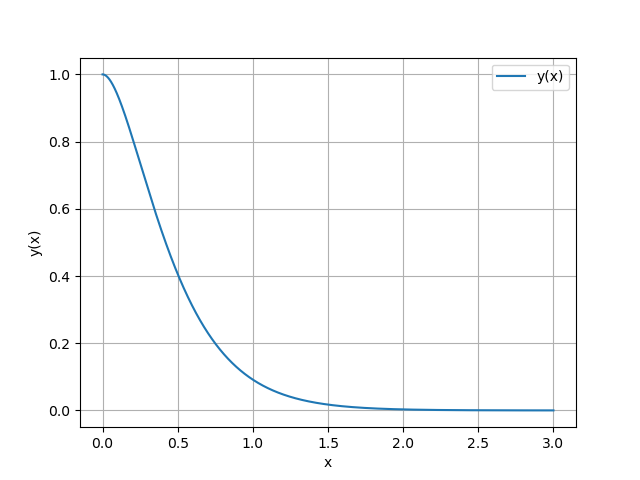
\includegraphics[width=1\linewidth]{2021/AE/1/figures/figure.png}
        \caption{Plot of y(x)}
    \label{fig:enter-label}
\end{figure}


%\end{document}






\pagebreak
\item\textbf{Question:}
The solution of second-order differential equation \\ $\frac{d^2y}{dx^2}+2\frac{dy}{dx}+y=0$ with boundary conditions $y(0)=1$ and $y(1)=3$.\\
\hfill{(GATE  2021 CE.26)}\\
\solution
\iffalse
\let\negmedspace\undefined
\let\negthickspace\undefined
\documentclass[journal,12pt,twocolumn]{IEEEtran}
\usepackage{xparse}
\usepackage{cite}
\usepackage{amsmath,amssymb,amsfonts,amsthm}
\usepackage{algorithmic}
\usepackage{graphicx}
\usepackage{textcomp}
\usepackage{xcolor}
\usepackage{txfonts}
\usepackage{listings}
\usepackage{enumitem}
\usepackage{mathtools}
\usepackage{gensymb}
\usepackage{comment}
\usepackage[breaklinks=true]{hyperref}
\usepackage{tkz-euclide}
\usepackage{listings}
\usepackage{gvv}
\def\inputGnumericTable{}
\usepackage[latin1]{inputenc}
\usepackage{color}
\usepackage{array}
\usepackage{longtable}
\usepackage{calc}
\usepackage{multirow}
\usepackage{hhline}
\usepackage{ifthen}
\usepackage{lscape}
\begin{enumerate}[label=\thechapter.\arabic*,ref=\thechapter.\theenumi]
\numberwithin{equation}{enumi}
\numberwithin{figure}{enumi}
\numberwithin{table}{enumi}
\item Laplace Transform of Partial Differentials\\
Let a function $y\brak{x,t}$ be defined for all $t>0$ and assumed to be bounded. Appling Laplace transform in t considering x as a parameter,
\begin{align}
 \mathcal{L}\brak{y\brak{x,t}} &= \int_{0}^{\infty}e^{-st}y\brak{x,t}dt\\
 &= Y\brak{x,s}
\end{align}
Let $\dfrac{\partial y\brak{x,t}}{\partial t}$ be $y_t\brak{x,t}$ and $\dfrac{\partial y\brak{x,t}}{\partial x}$ be $y_x\brak{x,t}$, then
\begin{align}
 \mathcal{L}\brak{y_t\brak{x,t}} &= \int_{0}^{\infty}e^{-st}y_t\brak{x,t}dt\\
 &= \left. e^{-st}y\brak{x,t}\right|_{0}^{\infty} + s\int_{0}^{\infty}e^{-st} y\brak{x,t} dt\\
 &= sY\brak{x,s} - y\brak{x,0} \label{L(y_t(x,t))}\\
 \mathcal{L}\brak{y_x\brak{x,t}} &= \int_{0}^{\infty}e^{-st}y_x\brak{x,t}dt\\
 &= \dfrac{d}{dx}\int_{0}^{\infty}e^{-st}y\brak{x,t}dt \label{L(y_x(x,t))}\\
 &= \dfrac{dY\brak{x,s}}{dx}
\end{align}
\item Laplace transform of f(t):
\begin{align}
        f(t)u(t)\system{L}&\int_{0}^{\infty}f(t)e^{-st}\; dt\\
        &=F(s)\label{lap transform}
\end{align}
\item Laplace transform of powers of $t$\\
        Let $f(t)=t^nu(t)$\\
From \eqref{lap transform},and considering $h=st$
\begin{align}
        F(s)&=\frac{1}{s^{n+1}}\int_{0}^{\infty}h^ne^{-h}\;dh\label{lap 1}\\
        (n-1)!&=\int_0^\infty e^{-t}t^{n-1}\;dt\text{ (Gamma function)}\label{gamma}
\end{align}
From \eqref{lap 1},\eqref{gamma}
\begin{align}
        F(s)&=\frac{n!}{s^{n+1}}\\
         t^nu(t)&\system{L}\frac{n!}{s^{n+1}}\label{lap exp}
\end{align}
\item Frequency shift property:\\
        Let $f(t)=y(t)e^{-at}u(t)$\\
From\eqref{lap transform},
\begin{align}
        F(s)&=\int_0^{\infty}y(t)e^{-(s+a)t}\;dt\\
         y(t)e^{-at}u(t)&\system{L}Y(s+a)\label{lap freq shift}
\end{align}
\item Inverse Laplace for partial fractions\\
From \eqref{lap exp},\eqref{lap freq shift} we get
\begin{align}
    &\frac{b}{(s+a)^n}\Large\xleftrightarrow{\mathcal{L}^{-1}}\frac{b}{(n-1)!}\cdot t^{n-1} e^{-at}\cdot u(t)\label{inv lap (partial fractions)}
\end{align}
\item Laplace transform of derivatives:\\
        Let $f(t)=y'(t)u(t)$\\
From \eqref{lap transform}, integration by parts,recursion
\begin{align}
        F(s)&=\int_{0}^\infty e^{-st}\; dy\\
        &=[y(t)e^{-st}]_0^\infty+s\int_0^\infty y(t)e^{-st}dt\\
        &=-y(0)+sY(s)\label{lap 2}
\end{align}
From\eqref{lap 2},recursion
\begin{align}
        y'(t)u(t)&\system{L}sY(s)-\int y'(t)\;dt\vert_{t=0}\\
        y^{(n)}(t)u(t)&\system{L}s^nY(s)-\sum\limits_{k=0}^{n-1}s^{(n-1-k)}y^{(k)}(0)\label{lap (derivatives)}
\end{align}
\end{enumerate}

\newtheorem{theorem}{Theorem}[section]
\newtheorem{problem}{Problem}
\newtheorem{proposition}{Proposition}[section]
\newtheorem{lemma}{Lemma}[section]
\newtheorem{corollary}[theorem]{Corollary}
\newtheorem{example}{Example}[section]
\newtheorem{definition}[problem]{Definition}
\newcommand{\BEQA}{\begin{eqnarray}}
\newcommand{\EEQA}{\end{eqnarray}}
\newcommand{\define}{\stackrel{\triangle}{=}}
\theoremstyle{remark}
\newtheorem{rem}{Remark}
\begin{document}

\bibliographystyle{IEEEtran}
\vspace{3cm}

\title{GATE-CE.26}
\author{EE23BTECH11046 - Poluri Hemanth$^{*}$}
\maketitle
\textbf{Question:}
The solution of second-order differential equation \\ $\frac{d^2y}{dx^2}+2\frac{dy}{dx}+y=0$ with boundary conditions $y(0)=1$ and $y(1)=3$.\\
\hfill{(GATE  2021 CE.26)}\\
\textbf{Solution:}
\fi
\begin{table}[h!]
    % Change address in github
        %%%%%%%%%%%%%%%%%%%%%%%%%%%%%%%%%%%%%%%%%%%%%%%%%%%%%%%%%%%%%%%%%%%%%%
%%                                                                  %%
%%  This is the header of a LaTeX2e file exported from Gnumeric.    %%
%%                                                                  %%
%%  This file can be compiled as it stands or included in another   %%
%%  LaTeX document. The table is based on the longtable package so  %%
%%  the longtable options (headers, footers...) can be set in the   %%
%%  preamble section below (see PRAMBLE).                           %%
%%                                                                  %%
%%  To include the file in another, the following two lines must be %%
%%  in the including file:                                          %%
%%        \def\inputGnumericTable{}                                 %%
%%  at the beginning of the file and:                               %%
%%        \input{name-of-this-file.tex}                             %%
%%  where the table is to be placed. Note also that the including   %%
%%  file must use the following packages for the table to be        %%
%%  rendered correctly:                                             %%
%%    \usepackage[latin1]{inputenc}                                 %%
%%    \usepackage{color}                                            %%
%%    \usepackage{array}                                            %%
%%    \usepackage{longtable}                                        %%
%%    \usepackage{calc}                                             %%
%%    \usepackage{multirow}                                         %%
%%    \usepackage{hhline}                                           %%
%%    \usepackage{ifthen}                                           %%
%%  optionally (for landscape tables embedded in another document): %%
%%    \usepackage{lscape}                                           %%
%%                                                                  %%
%%%%%%%%%%%%%%%%%%%%%%%%%%%%%%%%%%%%%%%%%%%%%%%%%%%%%%%%%%%%%%%%%%%%%%



%%  This section checks if we are begin input into another file or  %%
%%  the file will be compiled alone. First use a macro taken from   %%
%%  the TeXbook ex 7.7 (suggestion of Han-Wen Nienhuys).            %%
\def\ifundefined#1{\expandafter\ifx\csname#1\endcsname\relax}


%%  Check for the \def token for inputed files. If it is not        %%
%%  defined, the file will be processed as a standalone and the     %%
%%  preamble will be used.                                          %%
\ifundefined{inputGnumericTable}

%%  We must be able to close or not the document at the end.        %%
	\def\gnumericTableEnd{\end{document}}


%%%%%%%%%%%%%%%%%%%%%%%%%%%%%%%%%%%%%%%%%%%%%%%%%%%%%%%%%%%%%%%%%%%%%%
%%                                                                  %%
%%  This is the PREAMBLE. Change these values to get the right      %%
%%  paper size and other niceties.                                  %%
%%                                                                  %%
%%%%%%%%%%%%%%%%%%%%%%%%%%%%%%%%%%%%%%%%%%%%%%%%%%%%%%%%%%%%%%%%%%%%%%

	\documentclass[12pt%
			  %,landscape%
                    ]{report}
       \usepackage[latin1]{inputenc}
       \usepackage{fullpage}
       \usepackage{color}
       \usepackage{array}
       \usepackage{longtable}
       \usepackage{calc}
       \usepackage{multirow}
       \usepackage{hhline}
       \usepackage{ifthen}

	\begin{document}


%%  End of the preamble for the standalone. The next section is for %%
%%  documents which are included into other LaTeX2e files.          %%
\else

%%  We are not a stand alone document. For a regular table, we will %%
%%  have no preamble and only define the closing to mean nothing.   %%
    \def\gnumericTableEnd{}

%%  If we want landscape mode in an embedded document, comment out  %%
%%  the line above and uncomment the two below. The table will      %%
%%  begin on a new page and run in landscape mode.                  %%
%       \def\gnumericTableEnd{\end{landscape}}
%       \begin{landscape}


%%  End f the else clause for this file being \input.              %%
\fi

%%%%%%%%%%%%%%%%%%%%%%%%%%%%%%%%%%%%%%%%%%%%%%%%%%%%%%%%%%%%%%%%%%%%%%
%%                                                                  %%
%%  The rest is the gnumeric table, except for the closing          %%
%%  statement. Changes below will alter the table's appearance.     %%
%%                                                                  %%
%%%%%%%%%%%%%%%%%%%%%%%%%%%%%%%%%%%%%%%%%%%%%%%%%%%%%%%%%%%%%%%%%%%%%%

\providecommand{\gnumericmathit}[1]{#1} 
%%  Uncomment the next line if you would like your numbers to be in %%
%%  italics if they are italizised in the gnumeric table.           %%
%\renewcommand{\gnumericmathit}[1]{\mathit{#1}}
\providecommand{\gnumericPB}[1]%
{\let\gnumericTemp=\\#1\let\\=\gnumericTemp\hspace{0pt}}
 \ifundefined{gnumericTableWidthDefined}
        \newlength{\gnumericTableWidth}
        \newlength{\gnumericTableWidthComplete}
        \newlength{\gnumericMultiRowLength}
        \global\def\gnumericTableWidthDefined{}
 \fi
%% The following setting protects this code from babel shorthands.  %%
 \ifthenelse{\isundefined{\languageshorthands}}{}{\languageshorthands{english}}
%%  The default table format retains the relative column widths of  %%
%%  gnumeric. They can easily be changed to c, r or l. In that case %%
%%  you may want to comment out the next line and uncomment the one %%
%%  thereafter                                                      %%
\providecommand\gnumbox{\makebox[0pt]}
%%\providecommand\gnumbox[1][]{\makebox}

%% to adjust positions in multirow situations                       %%
\setlength{\bigstrutjot}{\jot}
\setlength{\extrarowheight}{\doublerulesep}

%%  The \setlongtables command keeps column widths the same across  %%
%%  pages. Simply comment out next line for varying column widths.  %%
\setlongtables

\setlength\gnumericTableWidth{%
	20pt+%
	40pt+%
	50pt+%	
0pt}
\def\gumericNumCols{3}
\setlength\gnumericTableWidthComplete{\gnumericTableWidth+%
         \tabcolsep*\gumericNumCols*2+\arrayrulewidth*\gumericNumCols}
\ifthenelse{\lengthtest{\gnumericTableWidthComplete > \linewidth}}%
         {\def\gnumericScale{1*\ratio{\linewidth-%
                        \tabcolsep*\gumericNumCols*2-%
                        \arrayrulewidth*\gumericNumCols}%
{\gnumericTableWidth}}}%
{\def\gnumericScale{2}}

%%%%%%%%%%%%%%%%%%%%%%%%%%%%%%%%%%%%%%%%%%%%%%%%%%%%%%%%%%%%%%%%%%%%%%
%%                                                                  %%
%% The following are the widths of the various columns. We are      %%
%% defining them here because then they are easier to change.       %%
%% Depending on the cell formats we may use them more than once.    %%
%%                                                                  %%
%%%%%%%%%%%%%%%%%%%%%%%%%%%%%%%%%%%%%%%%%%%%%%%%%%%%%%%%%%%%%%%%%%%%%%

\ifthenelse{\isundefined{\gnumericColA}}{\newlength{\gnumericColA}}{}\settowidth{\gnumericColA}{\begin{tabular}{@{}p{20pt*\gnumericScale}@{}}x\end{tabular}}
\ifthenelse{\isundefined{\gnumericColB}}{\newlength{\gnumericColB}}{}\settowidth{\gnumericColB}{\begin{tabular}{@{}p{40pt*\gnumericScale}@{}}x\end{tabular}}
\ifthenelse{\isundefined{\gnumericColC}}{\newlength{\gnumericColC}}{}\settowidth{\gnumericColC}{\begin{tabular}{@{}p{50pt*\gnumericScale}@{}}x\end{tabular}}

\begin{tabular}[c]{%
	b{\gnumericColA}%
	b{\gnumericColB}%
	b{\gnumericColC}%
	}

%%%%%%%%%%%%%%%%%%%%%%%%%%%%%%%%%%%%%%%%%%%%%%%%%%%%%%%%%%%%%%%%%%%%%%
%%  The longtable options. (Caption, headers... see Goosens, p.124) %%
%	\caption{The Table Caption.}             \\	%
% \hline	% Across the top of the table.
%%  The rest of these options are table rows which are placed on    %%
%%  the first, last or every page. Use \multicolumn if you want.    %%

%%  Header for the first page.                                      %%
%	\multicolumn{3}{c}{The First Header} \\ \hline 
%	\multicolumn{1}{c}{colTag}	%Column 1
%	&\multicolumn{1}{c}{colTag}	%Column 2
%	&\multicolumn{1}{c}{colTag}	\\ \hline %Last column
%	\endfirsthead

%%  The running header definition.                                  %%
%	\hline
%	\multicolumn{3}{l}{\ldots\small\slshape continued} \\ \hline
%	\multicolumn{1}{c}{colTag}	%Column 1
%	&\multicolumn{1}{c}{colTag}	%Column 2
%	&\multicolumn{1}{c}{colTag}	\\ \hline %Last column
%	\endhead

%%  The running footer definition.                                  %%
%	\hline
%	\multicolumn{3}{r}{\small\slshape continued\ldots} \\
%	\endfoot

%%  The ending footer definition.                                   %%
%	\multicolumn{3}{c}{That's all folks} \\ \hline 
%	\endlastfoot
%%%%%%%%%%%%%%%%%%%%%%%%%%%%%%%%%%%%%%%%%%%%%%%%%%%%%%%%%%%%%%%%%%%%%%
\hhline{|-|-|-}
	\multicolumn{1}{|p{\gnumericColA}|}%
	{\gnumericPB{\centering}\gnumbox{\textbf{Symbol}}}
	&\multicolumn{1}{p{\gnumericColB}|}%
	{\gnumericPB{\centering}\gnumbox{\textbf{Values}}}
	&\multicolumn{1}{p{\gnumericColC}|}%
	{\gnumericPB{\centering}\gnumbox{\textbf{Description}}}

\\
\hhline{|---|}
	\multicolumn{1}{|p{\gnumericColA}|}%
	{\gnumericPB{\centering}\gnumbox{$Y(s)$}}
	&\multicolumn{1}{p{\gnumericColB}|}%
	{\gnumericPB{\centering}\gnumbox{-}}
	&\multicolumn{1}{p{\gnumericColC}|}%
	{\gnumericPB{\centering}\gnumbox{$y$ in s domain}}

\\
\hhline{|---|}
        \multicolumn{1}{|p{\gnumericColA}|}%
	{\gnumericPB{\centering}\gnumbox{$y(x)$}}             
        &\multicolumn{1}{p{\gnumericColB}|}%
	{\gnumericPB{\centering}\gnumbox{-}}  
        &\multicolumn{1}{p{\gnumericColC}|}%
	{\gnumericPB{\centering}\gnumbox{$y$ in x domain}}

\\
\hhline{|---|}
        \multicolumn{1}{|p{\gnumericColA}|}%
        {\gnumericPB{\centering}\gnumbox{$y(0)$}}             
        &\multicolumn{1}{p{\gnumericColB}|}%
        {\gnumericPB{\centering}\gnumbox{1}}  
        &\multicolumn{1}{p{\gnumericColC}|}%
        {\gnumericPB{\centering}\gnumbox{$y$ at $x=0$}}
\\
\hhline{|---|}
        \multicolumn{1}{|p{\gnumericColA}|}%
        {\gnumericPB{\centering}\gnumbox{$y(1)$}}             
        &\multicolumn{1}{p{\gnumericColB}|}%
        {\gnumericPB{\centering}\gnumbox{3}}  
        &\multicolumn{1}{p{\gnumericColC}|}%
	{\gnumericPB{\centering}\gnumbox{$y(x)$ at $x=1$}}

\\
\hhline{|---|}
        \multicolumn{1}{|p{\gnumericColA}|}%
	{\gnumericPB{\centering}\gnumbox{$u(x)$}}             
        &\multicolumn{1}{p{\gnumericColB}|}%
	{\gnumericPB{\centering}\gnumbox{$=\begin{cases}
        1 & \text{if } x > 0\\
        0 &  o.w
    \end{cases}$}}  
        &\multicolumn{1}{p{\gnumericColC}|}%
        {\gnumericPB{\centering}\gnumbox{unit step function}}
\\
\hhline{|-|-|-|}
\end{tabular}

\ifthenelse{\isundefined{\languageshorthands}}{}{\languageshorthands{\languagename}}
\gnumericTableEnd

        \caption{Parameters}
        \label{tab:es.47}
\end{table}\\
Applying Laplace transform
\\From \ref{lap (derivatives)}
\begin{align}
	\frac{d^2y}{dx^2}+2\frac{dy}{dx}+y&\Large\xleftrightarrow{\mathcal{L}}s^2Y(s)-sy(0)-y'(0)+2sY(s)-2y(0)+Y(s)
\end{align}
\begin{align}
	Y(s)(s^2+2s+1)&=s-2-y'(0)
\end{align}
\begin{align}
	\Rightarrow Y(s)&=\frac{s-2-y'(0)}{s^2+2s+1}\\
	&=\frac{1}{s+1}-\frac{2+y'(0)}{(s+1)^2}\label{1ce.1}
\end{align}
For inversion of $Y(s)$ in partial fractions-
\\From \ref{inv lap (partial fractions)}
\begin{align}
	&\frac{b}{(s+a)^n}\system{L}\frac{b}{(n-1)!}\cdot x^{n-1} e^{-ax}\cdot u(x)\label{invce.26}
\end{align}
Applying Laplace inverse-\\
\\From \eqref{1ce.1},\eqref{invce.26}
\begin{align}
	y(x)&=\frac{1}{0!} e^{-x}\cdot u(x)-\frac{3+y'(0)}{1!}x\cdot e^{-x}\cdot u(x)\\
	&=(1-(3+y'(0))x)e^{-x}u(x)\label{yce.26}
\end{align}
From \eqref{yce.26},
\begin{align}
	y(1)&=(1-3-y'(0))e^{-1}\\
	3&=(1-3-y'(0))e^{-1}\\
	\Rightarrow y'(0)&=-(2+3e)\label{y'0ce.26}
\end{align}
From\eqref{y'0ce.26},\eqref{yce.26}
\begin{align}
	y(x)=(e^x+(3e-1)xe^{-x})u(x)
\end{align}
\\
\\
\\
\\
\\
\\
\\
\\
\\
\\
\\
\\
\\
\\
\begin{figure}[h!]
    \centering
    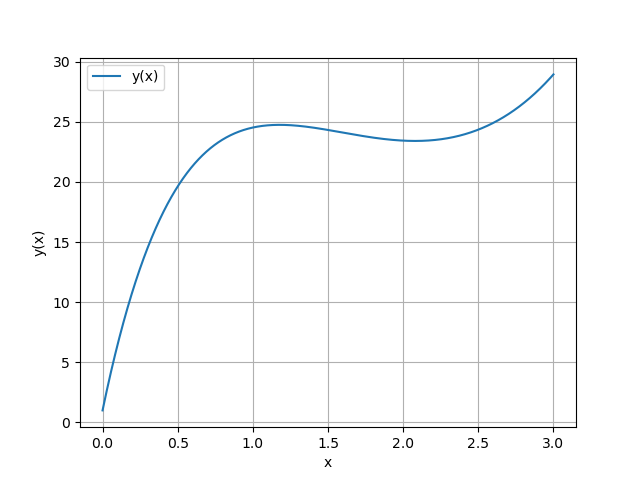
\includegraphics[width=1\linewidth]{2021/CE/26/figures/figure1.png}
        \caption{Plot of y(x)}
    \label{fig:enter-label}
\end{figure}


%\end{document}





\pagebreak
\item A system has a transfer function
\begin{align}
    G(s) = \frac{3e^{-4s}}{12s + 1}\nonumber
\end{align}
When a step-change of magnitude $M$ is given to the system input, the final value of the system output is measured to be 120. The value of M is \_\_\_\_\_.
\hfill(GATE 2021 CH Q52)\\
\solution
\iffalse
\let\negmedspace\undefined
\let\negthickspace\undefined
\documentclass[journal,12pt,twocolumn]{IEEEtran}
\usepackage{cite}
\usepackage{amsmath,amssymb,amsfonts,amsthm}
\usepackage{algorithmic}
\usepackage{graphicx}
\usepackage{textcomp}
\usepackage{xcolor}
\usepackage{txfonts}
\usepackage{listings}
\usepackage{enumitem}
\usepackage{mathtools}
\usepackage{gensymb}
\usepackage{comment}
\usepackage[breaklinks=true]{hyperref}
\usepackage{tkz-euclide} 
\usepackage{listings}
\usepackage{gvv}                            \usepackage{tikz}
\usepackage{circuitikz}
\def\inputGnumericTable{}                                
\usepackage[latin1]{inputenc}                            
\usepackage{color}                                       
\usepackage{array}                                       
\usepackage{longtable}                                   
\usepackage{calc}                              
\usepackage{tikz}
\usepackage{multirow}                                    
\usepackage{hhline}                                      
\usepackage{ifthen}                            
\usepackage{caption}
\usepackage{lscape}
\usepackage{amsmath}
\newtheorem{theorem}{Theorem}[section]
\newtheorem{problem}{Problem}
\newtheorem{proposition}{Proposition}[section]
\newtheorem{lemma}{Lemma}[section]
\newtheorem{corollary}[theorem]{Corollary}
\newtheorem{example}{Example}[section]
\newtheorem{definition}[problem]{Definition}
\newcommand{\BEQA}{\begin{eqnarray}}
\newcommand{\EEQA}{\end{eqnarray}}
\newcommand{\define}{\stackrel{\triangle}{=}}
\theoremstyle{remark}
\newtheorem{rem}{Remark}

\begin{document}

\bibliographystyle{IEEEtran}
\vspace{3cm}

\title{GATE 2021 CH Q52}
\author{EE23BTECH11009 - AROSHISH PRADHAN$^{*}$% <-this % stops a space
}
\maketitle
\newpage
\bigskip
\textbf{Question:} A system has a transfer function
\begin{align}
    G(s) = \frac{3e^{-4s}}{12s + 1}\nonumber
\end{align}
When a step-change of magnitude $M$ is given to the system input, the final value of the system output is measured to be 120. The value of M is \_\_\_\_\_.
\hfill(GATE 2021 CH Q52)\\
\solution
\fi
\begin{table}[!h]
    \centering
    \begin{tabular}{|c|c|c|}
    \hline
       \textbf{Symbol}  & \textbf{Value} & \textbf{Description}\\
    \hline
        $x(t)$ & $Mu(t)$ & Input Signal\\
    \hline
        $X(s)$ & $\frac{M}{s}$ & s-domain Input Signal\\
    \hline
        $y(t)$ &  & Output Signal\\
    \hline
        $Y(s)$ & & s-domain Output Signal\\
    \hline
       $G(s)$ & $\frac{3e^{-4s}}{12s + 1}$ & Transfer Function\\
    \hline
    \end{tabular}
    \caption{Given Parameters}
    \label{tab:1_gate.21.ch.52}
\end{table}


Given, input step-change:
\begin{align}
    x(t) &= Mu(t)\\
    u(t) &\system{L} \frac{1}{s}\\
    \implies X(s) &= \frac{M}{s}
\end{align}
Transfer Function:
\begin{align}
    G(s) &= \frac{Y(s)}{X(s)} = \frac{3e^{-4s}}{12s + 1}\\
    \implies Y(s) &= \frac{3e^{-4s}}{12s + 1}\frac{M}{s}
\end{align}
$\therefore$ system output
\begin{align}
     \lim_{s\rightarrow0}sY(s) &= 120\\
    \implies \lim_{s\rightarrow0}\brak{\frac{3e^{-4s}}{12s + 1}M} &= 120\\
    \implies 3M &= 120\\
    \implies M &= 40
\end{align}

\begin{figure}
    \centering
    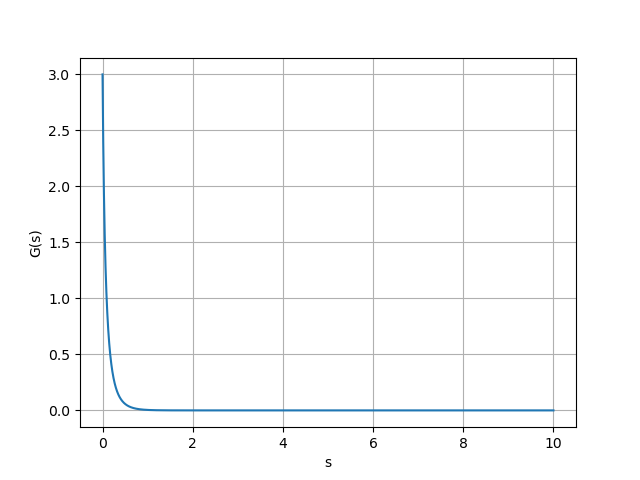
\includegraphics[width = \columnwidth]{2021/CH/52/figs/assign9.png}
	\caption{Plot of $G(s)$ vs $s$}
    \label{fig:1_gate.21.ch.52}
\end{figure}
%\end{document}

\pagebreak
\item The Bode magnitude plot for the transfer function $\frac{V_o(s)}{V_i(s)}$ of the circuit is as shown. The value of R is \_\_\_\_\_$\Omega$. \hfill(GATE 2021 EE Q20)
\begin{figure}[!ht]
    \centering
    \begin{circuitikz}
   \draw(0,0) to [R](2,0);
   % \draw (2,0) -- (2.5,0);
   \draw(2,0) to [L] (4,0);
   % \draw (5,0) to (5,0);
   \draw (4,0) to [C] (4,-2);
   \draw(4,-2)  to (0,-2);
   \draw (4,0) -- (5,0);
   \draw (4,-2)to (5,-2);
   \node[circle,fill,inner sep=1pt] at (0,0) {};
   \node[circle,fill,inner sep=1pt] at (5,0) {};
   \node[circle,fill,inner sep=1pt] at (5,-2) {};
   \node[circle,fill,inner sep=1pt] at (0,-2) {};
   \draw[->](0,-1.85) to (0,-0.15);
   \draw[->](5,-1.85) to (5,-0.15);
   \node at (0.3,-1) {$V_i$};
   \node at (5.5,-1) {$V_o$};

   \node at (1,0.5) {$R$};
   \node at (3,0.5) {$1mH$};
   \node at (2.8,-1) {$250\micro F$};\node[circle,fill,inner sep=1pt] at (0,0) {};
\end{circuitikz}

\end{figure}
\begin{figure}[!ht]
    \centering
    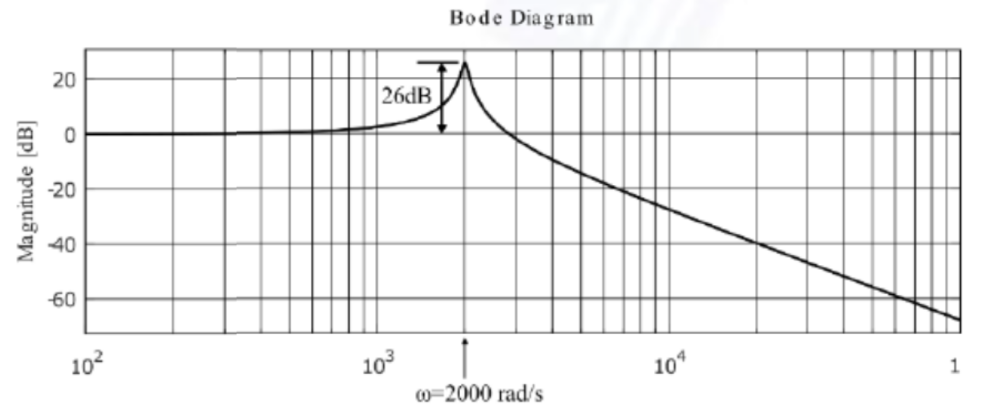
\includegraphics[width=\columnwidth]{2021/EE/20/figs/bode.png}
\end{figure}
\solution
\iffalse
\let\negmedspace\undefined
\let\negthickspace\undefined
\documentclass[journal,12pt,twocolumn]{IEEEtran}
\usepackage{cite}
\usepackage{amsmath,amssymb,amsfonts,amsthm}
\usepackage{algorithmic}
\usepackage{textcomp}
\usepackage{xcolor}
\usepackage{txfonts}
\usepackage{listings}
\usepackage{enumitem}
\usepackage{mathtools}
\usepackage{gensymb}
\usepackage{comment}
\usepackage[breaklinks=true]{hyperref}
\usepackage{tkz-euclide} 
\usepackage{listings}
\usepackage{gvv}                            \usepackage{tikz}
\usepackage{circuitikz}
\def\inputGnumericTable{}                                
\usepackage[latin1]{inputenc}                            
\usepackage{color}                                       
\usepackage{array}                                       
\usepackage{longtable}                                   
\usepackage{calc}                              
\usepackage{tikz}
\usepackage{multirow}                                    
\usepackage{hhline}                                      
\usepackage{ifthen}                            
\usepackage{caption}
\usepackage{lscape}
\usepackage{amsmath}
\newtheorem{theorem}{Theorem}[section]
\newtheorem{problem}{Problem}
\newtheorem{proposition}{Proposition}[section]
\newtheorem{lemma}{Lemma}[section]
\newtheorem{corollary}[theorem]{Corollary}
\newtheorem{example}{Example}[section]
\newtheorem{definition}[problem]{Definition}
\newcommand{\BEQA}{\begin{eqnarray}}
\newcommand{\EEQA}{\end{eqnarray}}
\newcommand{\define}{\stackrel{\triangle}{=}}
\theoremstyle{remark}
\newtheorem{rem}{Remark}

\begin{document}

\bibliographystyle{IEEEtran}
\vspace{3cm}

\title{GATE 2021 EE.20}
\author{EE23BTECH11010 - VENKATESH BANDAWAR$^{*}$% <-this % stops a space
}
\maketitle
\newpage
\bigskip
\textbf{Question:} The Bode magnitude plot for the transfer function $\frac{V_o(s)}{V_i(s)}$ of the circuit is as shown. The value of R is \_\_\_\_\_$\Omega$. \hfill(GATE 2021 EE Q20)
\begin{figure}[!ht]
    \centering
    \begin{circuitikz}
   \draw(0,0) to [R](2,0);
   % \draw (2,0) -- (2.5,0);
   \draw(2,0) to [L] (4,0);
   % \draw (5,0) to (5,0);
   \draw (4,0) to [C] (4,-2);
   \draw(4,-2)  to (0,-2);
   \draw (4,0) -- (5,0);
   \draw (4,-2)to (5,-2);
   \node[circle,fill,inner sep=1pt] at (0,0) {};
   \node[circle,fill,inner sep=1pt] at (5,0) {};
   \node[circle,fill,inner sep=1pt] at (5,-2) {};
   \node[circle,fill,inner sep=1pt] at (0,-2) {};
   \draw[->](0,-1.85) to (0,-0.15);
   \draw[->](5,-1.85) to (5,-0.15);
   \node at (0.3,-1) {$V_i$};
   \node at (5.5,-1) {$V_o$};

   \node at (1,0.5) {$R$};
   \node at (3,0.5) {$1mH$};
   \node at (2.8,-1) {$250\micro F$};\node[circle,fill,inner sep=1pt] at (0,0) {};
\end{circuitikz}

\end{figure}
\begin{figure}[!ht]
    \centering
    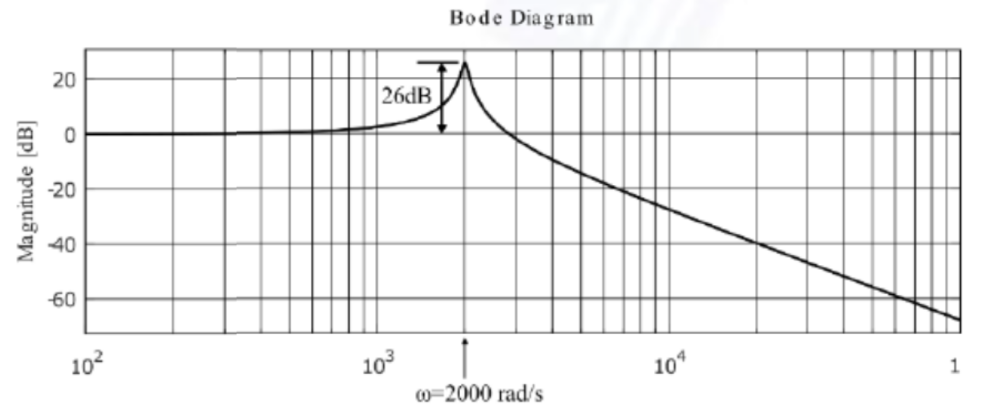
\includegraphics[width=\columnwidth]{2021/EE/20/figs/bode.png}
\end{figure}
\solution
\fi
\begin{table}[!ht]
    \centering
    \begin{tabular}{|c|c|c|}
\hline
    \textbf{Parameter} & \textbf{Description} & \textbf{Value} \\
    \hline
    $C$ & Capacitance & $250\micro F$\\
    \hline
    $L$ & Inductor & $1mH$\\
    \hline
    $I$ & Current &  \\
    \hline
    $I(0)$ & Initial Current & 0A \\
    \hline
    $V_o$ & Voltage across capacitor & \\
    \hline 
    $V_i$ & Input Voltage & \\
    \hline 
    $T(s)$ & Transfer Function & $\frac{V_o(s)}{V_i(s)}$\\
    \hline
    \end{tabular}

    \caption{Given Parameters table}
    \label{Given Parameters table_2021_EE_20}
\end{table}
Applying KVL,
\begin{align}
    V_i - R I - L\frac{dI}{dt} - \frac{\int I dt}{C} = 0
\end{align}
Taking Laplace Transform ,
\begin{align}
    V_i(s) &- RI(s) - LsI(s) + LI(0^+) - \frac{I(s)}{sC} = 0\\
    I(s) &= \frac{V_i(s) + LI(0)}{R + sL + \frac{1}{sC}}\\
    V_o(s) &= \frac{V_i(s) + LI(0)}{RsC + s^2LC + 1}
\end{align}
Substituting $I(0) = 0$ and $s = j\omega$,
\begin{align}
    \frac{V_o(j\omega)}{V_i(j\omega)} &= \frac{1}{\omega RCj -\omega^2LC + 1} 
\end{align}
$\because$ Magnitude in bode plot = $20\log \abs{T(s)}$\\
From given graph,At $\omega = 2000$
\begin{align}
    26 &= 20 \log \abs{\frac{V_o}{V_i}}\\
    \abs{\frac{V_o}{V_i}} &= 20
\end{align}
\begin{align}
    \implies 20 &= \abs{\frac{1}{\omega RCj -\omega^2LC + 1}} \\
    R &= 0.1 \Omega
\end{align}
\begin{figure}[!h]
    \centering
    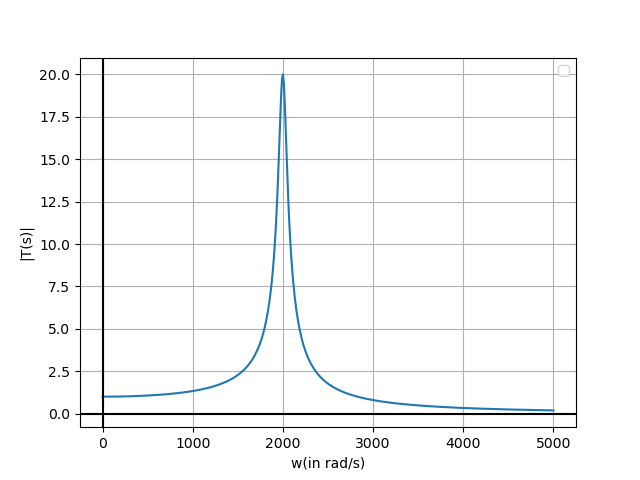
\includegraphics[width=\columnwidth]{2021/EE/20/figs/frequency_response.png}
    \caption{Frequency response of $V_o$}
    \label{frequency_response_2021_EE_20}
\end{figure}
%\end{document}

\pagebreak
\item Consider a system with transfer-function $G\brak{s}=\frac{2}{s+1}$. A unit-step function $\mu\brak{t}$ is applied to the system, which results in an output y\brak{t}. 

If $e\brak{t}=y\brak{t}-\mu\brak{t}$ then $ \lim_{t\to\infty} e(t)$ is\rule{1.5cm}{0.15mm}.
\solution
\iffalse
\let\negmedspace\undefined
\let\negthickspace\undefined
\documentclass[journal,12pt,twocolumn]{IEEEtran}
\usepackage{cite}
\usepackage{amsmath,amssymb,amsfonts,amsthm}
\usepackage{algorithmic}
\usepackage{graphicx}
\usepackage{textcomp}
\usepackage{xcolor}
\usepackage{txfonts}
\usepackage{listings}
\usepackage{enumitem}
\usepackage{mathtools}
\usepackage{gensymb}
\usepackage{comment}
\usepackage[breaklinks=true]{hyperref}
\usepackage{tkz-euclide} 
\usepackage{listings}
\usepackage{gvv}                                        
\def\inputGnumericTable{}                                 
\usepackage[latin1]{inputenc}                                
\usepackage{color}                                            
\usepackage{array}                                            
\usepackage{longtable}                                       
\usepackage{calc}                                             
\usepackage{multirow}                                         
\usepackage{hhline}                                           
\usepackage{ifthen}                                           
\usepackage{lscape}
\newtheorem{theorem}{Theorem}[section]
\newtheorem{problem}{Problem}
\newtheorem{proposition}{Proposition}[section]
\newtheorem{lemma}{Lemma}[section]
\newtheorem{corollary}[theorem]{Corollary}
\newtheorem{example}{Example}[section]
\newtheorem{definition}[problem]{Definition}
\newcommand{\BEQA}{\begin{eqnarray}}
\newcommand{\EEQA}{\end{eqnarray}}
\newcommand{\define}{\stackrel{\triangle}{=}}
\theoremstyle{remark}
\usepackage{circuitikz}
\newtheorem{rem}{Remark}
\begin{document}
\parindent 0px

\bibliographystyle{IEEEtran}
\vspace{3cm}

\title{Assignment\\[1ex]GATE-IN-46}
\author{EE23BTECH11034 - Prabhat Kukunuri$^{}$% <-this % stops a space
}
\maketitle
\newpage
\bigskip

\renewcommand{\thefigure}{\theenumi}
\renewcommand{\thetable}{\theenumi}
\section{Question}
Consider a system with transfer-function $G\brak{s}=\frac{2}{s+1}$. A unit-step function $\mu\brak{t}$ is applied to the system, which results in an output y\brak{t}. 

If $e\brak{t}=y\brak{t}-\mu\brak{t}$ then $ \lim_{t\to\infty} e(t)$ is\rule{1.5cm}{0.15mm}.

\solution
\fi
\begin{table}[h]
    \centering
    \begin{tabular}{|p{1cm}|p{3.00cm}|p{3.50cm}|}
    \hline
    Symbol&Value&Description\\ \hline
    $$G\brak{s}$$&$$\frac{2}{s+1}$$&$$\text{Transfer function}$$\\\hline
    $$e\brak{t}$$&$$y\brak{t}-\mu\brak{t}$$&$$\text{Function of y\brak{t} and $\mu\brak{t}$}$$\\\hline
    $$Y\brak{s}$$&$$G\brak{s}\times U\brak{s}$$&Convolution in $t$ domain is multiplication in $s$ domain.\\\hline
    $$\mu\brak{t}$$&$$\begin{cases}
    0&\text{if t$<$0}\\
    1&\text{if t$>$0}
    \end{cases}$$&$$\text{Unit step function}$$\\\hline
    \end{tabular}
    \caption{Variable description}
    \label{tab:GATE.2021.IN.46.1}
\end{table}\\
Applying Laplace transform on $\mu\brak{t}$
\begin{align}
    &\mu\brak{t}\system{L}U\brak{s}\\
    &U\brak{s}=\frac{1}{s}\\
    &Y\brak{s}=\brak{\frac{2}{s+1}}\brak{\frac{1}{s}}\\
    &Y\brak{s}=\frac{2}{s}-\frac{2}{s+1}
\end{align}
The inverse Laplace transform of $\frac{a}{s+b}$ is $ae^{-bt}\mu\brak{t}$
\begin{align}
    &y\brak{t}=2\mu\brak{t}-2e^{-t}\mu\brak{t}\\
    &e\brak{t}=\mu\brak{t}\brak{1-2e^{-t}}\\
    &\lim_{t\to\infty}e\brak{t}=\lim_{t\to\infty}\mu\brak{t}\brak{1-2e^{-t}}\\
    &\lim_{t\to\infty}e\brak{t}=1
\end{align}
%\end{document}

\pagebreak
\item  Solution of differential equation $y'' + y'+ 0.25y = 0$ with initial values $y(0) = 3$ and $y'(0) = -3.5$ is
\begin{enumerate}
    \item[(A)] $ y = (3-2x)e^{0.5x} $
    \item[(B)] $ y = (3-2x)e^{-0.25x}$
    \item[(C)] $ y = (3-2x)e^{-0.5x}$
    \item[(D)] $ y = (2-3x)e^{-0.5x}$
\end{enumerate} 
\hfill(GATE AG 2021) \\
\solution
\iffalse
\let\negmedspace\undefined
\let\negthickspace\undefined
\documentclass[journal,12pt,twocolumn]{IEEEtran}
\usepackage{cite}
\usepackage{amsmath,amssymb,amsfonts,amsthm}
\usepackage{algorithmic}
\usepackage{graphicx}
\usepackage{textcomp}
\usepackage{xcolor}
\usepackage{txfonts}
\usepackage{listings}
\usepackage{enumitem}
\usepackage{mathtools}
\usepackage{gensymb}
\usepackage{comment}
\usepackage[breaklinks=true]{hyperref}
\usepackage{tkz-euclide} 
\usepackage{listings}
\usepackage{gvv}                                        
\def\inputGnumericTable{}                                 
\usepackage[latin1]{inputenc}                                
\usepackage{color}                                            
\usepackage{array}                                            
\usepackage{longtable}                                       
\usepackage{calc}                                             
\usepackage{multirow}                                         
\usepackage{hhline}                                           
\usepackage{ifthen}                                           
\usepackage{lscape}
\usepackage{amsmath}
\usepackage{caption}

\newtheorem{theorem}{Theorem}[section]
\newtheorem{problem}{Problem}
\newtheorem{proposition}{Proposition}[section]
\newtheorem{lemma}{Lemma}[section]
\newtheorem{corollary}[theorem]{Corollary}
\newtheorem{example}{Example}[section]
\newtheorem{definition}[problem]{Definition}
\newcommand{\BEQA}{\begin{eqnarray}}
\newcommand{\EEQA}{\end{eqnarray}}
\newcommand{\define}{\stackrel{\triangle}{=}}
\theoremstyle{remark}
\newtheorem{rem}{Remark}
\begin{document}

\bibliographystyle{IEEEtran}
\vspace{3cm}

\title{GATE: AG-26 2021}
\author{EE23BTECH11038 - Rohith Madhani$^{*}$% <-this % stops a space
}
\maketitle
\newpage
\bigskip
\renewcommand{\thefigure}{\theenumi}
\renewcommand{\thetable}{\theenumi}

\textbf{Question :} Solution of differential equation $y'' + y'+ 0.25y = 0$ with initial values $y(0) = 3$ and $y'(0) = -3.5$ is
\begin{enumerate}
    \item[(A)] $ y = (3-2x)e^{0.5x} $
    \item[(B)] $ y = (3-2x)e^{-0.25x}$
    \item[(C)] $ y = (3-2x)e^{-0.5x}$
    \item[(D)] $ y = (2-3x)e^{-0.5x}$
\end{enumerate} 
\hfill(GATE AG 2021) \\
\solution
\fi

\begin{table}[!h] 
    \centering
    %%%%%%%%%%%%%%%%%%%%%%%%%%%%%%%%%%%%%%%%%%%%%%%%%%%%%%%%%%%%%%%%%%%%%%
%%                                                                  %%
%%  This is the header of a LaTeX2e file exported from Gnumeric.    %%
%%                                                                  %%
%%  This file can be compiled as it stands or included in another   %%
%%  LaTeX document. The table is based on the longtable package so  %%
%%  the longtable options (headers, footers...) can be set in the   %%
%%  preamble section below (see PRAMBLE).                           %%
%%                                                                  %%
%%  To include the file in another, the following two lines must be %%
%%  in the including file:                                          %%
%%        \def\inputGnumericTable{}                                 %%
%%  at the beginning of the file and:                               %%
%%        \input{name-of-this-file.tex}                             %%
%%  where the table is to be placed. Note also that the including   %%
%%  file must use the following packages for the table to be        %%
%%  rendered correctly:                                             %%
%%    \usepackage[latin1]{inputenc}                                 %%
%%    \usepackage{color}                                            %%
%%    \usepackage{array}                                            %%
%%    \usepackage{longtable}                                        %%
%%    \usepackage{calc}                                             %%
%%    \usepackage{multirow}                                         %%
%%    \usepackage{hhline}                                           %%
%%    \usepackage{ifthen}                                           %%
%%  optionally (for landscape tables embedded in another document): %%
%%    \usepackage{lscape}                                           %%
%%                                                                  %%
%%%%%%%%%%%%%%%%%%%%%%%%%%%%%%%%%%%%%%%%%%%%%%%%%%%%%%%%%%%%%%%%%%%%%%



%%  This section checks if we are begin input into another file or  %%
%%  the file will be compiled alone. First use a macro taken from   %%
%%  the TeXbook ex 7.7 (suggestion of Han-Wen Nienhuys).            %%
\def\ifundefined#1{\expandafter\ifx\csname#1\endcsname\relax}


%%  Check for the \def token for inputed files. If it is not        %%
%%  defined, the file will be processed as a standalone and the     %%
%%  preamble will be used.                                          %%
\ifundefined{inputGnumericTable}

%%  We must be able to close or not the document at the end.        %%
	\def\gnumericTableEnd{\end{document}}


%%%%%%%%%%%%%%%%%%%%%%%%%%%%%%%%%%%%%%%%%%%%%%%%%%%%%%%%%%%%%%%%%%%%%%
%%                                                                  %%
%%  This is the PREAMBLE. Change these values to get the right      %%
%%  paper size and other niceties.                                  %%
%%                                                                  %%
%%%%%%%%%%%%%%%%%%%%%%%%%%%%%%%%%%%%%%%%%%%%%%%%%%%%%%%%%%%%%%%%%%%%%%

	\documentclass[12pt%
			  %,landscape%
                    ]{report}
       \usepackage[latin1]{inputenc}
       \usepackage{fullpage}
       \usepackage{color}
       \usepackage{array}
       \usepackage{longtable}
       \usepackage{calc}
       \usepackage{multirow}
       \usepackage{hhline}
       \usepackage{ifthen}

	\begin{document}


%%  End of the preamble for the standalone. The next section is for %%
%%  documents which are included into other LaTeX2e files.          %%
\else

%%  We are not a stand alone document. For a regular table, we will %%
%%  have no preamble and only define the closing to mean nothing.   %%
    \def\gnumericTableEnd{}

%%  If we want landscape mode in an embedded document, comment out  %%
%%  the line above and uncomment the two below. The table will      %%
%%  begin on a new page and run in landscape mode.                  %%
%       \def\gnumericTableEnd{\end{landscape}}
%       \begin{landscape}


%%  End of the else clause for this file being \input.              %%
\fi

%%%%%%%%%%%%%%%%%%%%%%%%%%%%%%%%%%%%%%%%%%%%%%%%%%%%%%%%%%%%%%%%%%%%%%
%%                                                                  %%
%%  The rest is the gnumeric table, except for the closing          %%
%%  statement. Changes below will alter the table's appearance.     %%
%%                                                                  %%
%%%%%%%%%%%%%%%%%%%%%%%%%%%%%%%%%%%%%%%%%%%%%%%%%%%%%%%%%%%%%%%%%%%%%%

\providecommand{\gnumericmathit}[1]{#1} 
%%  Uncomment the next line if you would like your numbers to be in %%
%%  italics if they are italizised in the gnumeric table.           %%
%\renewcommand{\gnumericmathit}[1]{\mathit{#1}}
\providecommand{\gnumericPB}[1]%
{\let\gnumericTemp=\\#1\let\\=\gnumericTemp\hspace{0pt}}
 \ifundefined{gnumericTableWidthDefined}
        \newlength{\gnumericTableWidth}
        \newlength{\gnumericTableWidthComplete}
        \newlength{\gnumericMultiRowLength}
        \global\def\gnumericTableWidthDefined{}
 \fi
%% The following setting protects this code from babel shorthands.  %%
 \ifthenelse{\isundefined{\languageshorthands}}{}{\languageshorthands{english}}
%%  The default table format retains the relative column widths of  %%
%%  gnumeric. They can easily be changed to c, r or l. In that case %%
%%  you may want to comment out the next line and uncomment the one %%
%%  thereafter                                                      %%
\providecommand\gnumbox{\makebox[0pt]}
%%\providecommand\gnumbox[1][]{\makebox}

%% to adjust positions in multirow situations                       %%
\setlength{\bigstrutjot}{\jot}
\setlength{\extrarowheight}{\doublerulesep}

%%  The \setlongtables command keeps column widths the same across  %%
%%  pages. Simply comment out next line for varying column widths.  %%
\setlongtables

\setlength\gnumericTableWidth{%
	44pt+%
	200pt+%
	60pt+%
0pt}
\def\gumericNumCols{3}
\setlength\gnumericTableWidthComplete{\gnumericTableWidth+%
         \tabcolsep*\gumericNumCols*2+\arrayrulewidth*\gumericNumCols}
\ifthenelse{\lengthtest{\gnumericTableWidthComplete > \linewidth}}%
         {\def\gnumericScale{1*\ratio{\linewidth-%
                        \tabcolsep*\gumericNumCols*2-%
                        \arrayrulewidth*\gumericNumCols}%
{\gnumericTableWidth}}}%
{\def\gnumericScale{1}}

%%%%%%%%%%%%%%%%%%%%%%%%%%%%%%%%%%%%%%%%%%%%%%%%%%%%%%%%%%%%%%%%%%%%%%
%%                                                                  %%
%% The following are the widths of the various columns. We are      %%
%% defining them here because then they are easier to change.       %%
%% Depending on the cell formats we may use them more than once.    %%
%%                                                                  %%
%%%%%%%%%%%%%%%%%%%%%%%%%%%%%%%%%%%%%%%%%%%%%%%%%%%%%%%%%%%%%%%%%%%%%%

\ifthenelse{\isundefined{\gnumericColA}}{\newlength{\gnumericColA}}{}\settowidth{\gnumericColA}{\begin{tabular}{@{}p{44pt*\gnumericScale}@{}}t\end{tabular}}
\ifthenelse{\isundefined{\gnumericColB}}{\newlength{\gnumericColB}}{}\settowidth{\gnumericColB}{\begin{tabular}{@{}p{200pt*\gnumericScale}@{}}t\end{tabular}}
\ifthenelse{\isundefined{\gnumericColC}}{\newlength{\gnumericColC}}{}\settowidth{\gnumericColC}{\begin{tabular}{@{}p{60pt*\gnumericScale}@{}}t\end{tabular}}

\begin{tabular}[c]{%
	b{\gnumericColA}%
	b{\gnumericColB}%
	b{\gnumericColC}%
	}

%%%%%%%%%%%%%%%%%%%%%%%%%%%%%%%%%%%%%%%%%%%%%%%%%%%%%%%%%%%%%%%%%%%%%%
%%  The longtable options. (Caption, headers... see Goosens, p.124) %%
%	\caption{The Table Caption.}             \\	%
% \hline	% Across the top of the table.
%%  The rest of these options are table rows which are placed on    %%
%%  the first, last or every page. Use \multicolumn if you want.    %%

%%  Header for the first page.                                      %%
%	\multicolumn{3}{c}{The First Header} \\ \hline 
%	\multicolumn{1}{c}{colTag}	%Column 1
%	&\multicolumn{1}{c}{colTag}	%Column 2
%	&\multicolumn{1}{c}{colTag}	\\ \hline %Last column
%	\endfirsthead

%%  The running header definition.                                  %%
%	\hline
%	\multicolumn{3}{l}{\ldots\small\slshape continued} \\ \hline
%	\multicolumn{1}{c}{colTag}	%Column 1
%	&\multicolumn{1}{c}{colTag}	%Column 2
%	&\multicolumn{1}{c}{colTag}	\\ \hline %Last column
%	\endhead

%%  The running footer definition.                                  %%
%	\hline
%	\multicolumn{3}{r}{\small\slshape continued\ldots} \\
%	\endfoot

%%  The ending footer definition.                                   %%
%	\multicolumn{3}{c}{That's all folks} \\ \hline 
%	\endlastfoot
%%%%%%%%%%%%%%%%%%%%%%%%%%%%%%%%%%%%%%%%%%%%%%%%%%%%%%%%%%%%%%%%%%%%%%

\hhline{|-|-|-|}
	 \multicolumn{1}{|p{\gnumericColA}|}%
	{\gnumericPB{\centering}\gnumbox{Parameter}}
	&\multicolumn{1}{p{\gnumericColB}|}%
	{\gnumericPB{\centering}\gnumbox{Description}}
	&\multicolumn{1}{p{\gnumericColC}|}%
	{\gnumericPB{\centering}\gnumbox{Value}}
\\
\hhline{|-|-|-|}
	 \multicolumn{1}{|p{\gnumericColA}|}%
	{\gnumericPB{\centering}\gnumbox{$y(t)$}}
	&\multicolumn{1}{p{\gnumericColB}|}%
	{\gnumericPB{\centering}\gnumbox{y in time domain}}
	&\multicolumn{1}{p{\gnumericColC}|}%
	{\gnumericPB{\centering}\gnumbox{?}}
\\
\hhline{|-|-|-|}
	 \multicolumn{1}{|p{\gnumericColA}|}%
	{\gnumericPB{\centering}\gnumbox{$y(0)$}}
	&\multicolumn{1}{p{\gnumericColB}|}%
	{\gnumericPB{\centering}\gnumbox{$y$ at $t=0$}}
	&\multicolumn{1}{p{\gnumericColC}|}%
	{\gnumericPB{\centering}\gnumbox{3}}
\\
\hhline{|-|-|-|}
	 \multicolumn{1}{|p{\gnumericColA}|}%
	{\gnumericPB{\centering}\gnumbox{$y'(0)$}}
	&\multicolumn{1}{p{\gnumericColB}|}%
	{\gnumericPB{\centering}\gnumbox{$y'$ at $t=0$}}
	&\multicolumn{1}{p{\gnumericColC}|}%
	{\gnumericPB{\centering}\gnumbox{-3.5}}
\\
\hhline{|-|-|-|}
\end{tabular}

\ifthenelse{\isundefined{\languageshorthands}}{}{\languageshorthands{\languagename}}
\gnumericTableEnd
    \caption{Given parameters}
    \label{table:gate21ag26}
\end{table}
By applying laplace transform to the differential equation,
\begin{align}
    y''+y'+0.25y &\Large\xleftrightarrow{\mathcal{L}} s^2Y(s)-sy(0)-y'(0)+sY(s)-y(0)+0.25Y(s)
\end{align}

\begin{align}
    Y(s)(s^2 + s + 0.25) &= 3s - 0.5 \\
    \implies Y(s) &= \frac{3s-0.5}{s^2 + s + 0.25} \\
    &= \frac{3}{s+0.5} - \frac{2}{(s+0.5)^2};Re(s) > -0.5 \label{parfrac}
\end{align}

As we know,
\begin{align}
    \frac{b}{(s+a)^n} &\Large\xleftrightarrow{\mathcal{L}^{-1}}\frac{b}{(n-1)!} t^{n-1} e^{-at} u(t)
\end{align}

By taking inverse laplace of \eqref{parfrac}, we get
\begin{align}
    y(t) &= \frac{3}{0!}e^{-0.5t}u(t)-\frac{2}{1!}te^{-0.5t}u(t) \\
    \implies y(t) &= \sbrak{(3-2x)e^{-0.5t}}u(t)
\end{align}
Hence the correct answer is option (C)
\newpage

\begin{figure}[t]
    \centering
    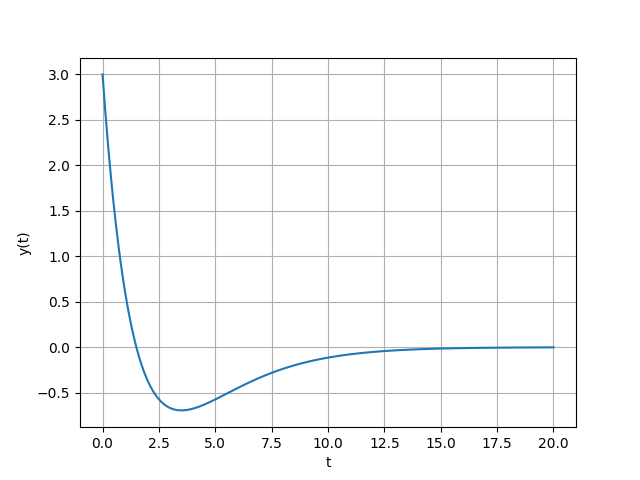
\includegraphics[width=\columnwidth]{2021/AG/26/figs/fig1.png}
    \caption{$y(t) = \sbrak{(3-2t)e^{-0.5t}}u(t)$}
    \label{fig:gate21ag26}
\end{figure}

%\end{document}

\pagebreak
\item Consider the following first order partial differential equation, also known as the transport equation
\begin{align*}
\frac{\partial y\brak{x,t}}{\partial t}+5\frac{\partial y\brak{x,t}}{\partial x}&=0
\end{align*}
with initial conditions given by $y(x, 0) = \sin x,-\infty < x < \infty$. The value of $y(x, t)$ at $x = \pi$ and $t=\frac{\pi}{6}$ is  \rule{1cm}{0.15mm}.
\begin{enumerate}[label=(\Alph*)]
\item 1
\item 2
\item 0
\item 0.5
\end{enumerate}
\hfill(GATE 2021 BM Q28)\\
\solution
\iffalse
\let\negmedspace\undefined
\let\negthickspace\undefined
\documentclass[journal,12pt,twocolumn]{IEEEtran}
\usepackage{cite}
\usepackage{amsmath,amssymb,amsfonts,amsthm}
\usepackage{algorithmic}
\usepackage{graphicx}
\usepackage{textcomp}
\usepackage{xcolor}
\usepackage{txfonts}
\usepackage{listings}
\usepackage{enumitem}
\usepackage{mathtools}
\usepackage{gensymb}
\usepackage{comment}
\usepackage[breaklinks=true]{hyperref}
\usepackage{tkz-euclide} 
\usepackage{listings}
\usepackage{gvv}                                        
\def\inputGnumericTable{}                                 
\usepackage[latin1]{inputenc}                                
\usepackage{color}                                            
\usepackage{array}                                            
\usepackage{longtable}                                       
\usepackage{calc}                                             
\usepackage{multirow}                                         
\usepackage{hhline}                                           
\usepackage{ifthen}                                           
\usepackage{lscape}
\newtheorem{theorem}{Theorem}[section]
\newtheorem{problem}{Problem}
\newtheorem{proposition}{Proposition}[section]
\newtheorem{lemma}{Lemma}[section]
\newtheorem{corollary}[theorem]{Corollary}
\newtheorem{example}{Example}[section]
\newtheorem{definition}[problem]{Definition}
\newcommand{\BEQA}{\begin{eqnarray}}
\newcommand{\EEQA}{\end{eqnarray}}
\newcommand{\define}{\stackrel{\triangle}{=}}
\theoremstyle{remark}
\newtheorem{rem}{Remark}
\begin{document}

\bibliographystyle{IEEEtran}
\vspace{3cm}

\title{GATE: BM - 28.2021}
\author{EE23BTECH11224 - Sri Krishna Prabhas Yadla$^{*}$% <-this % stops a space
}
\maketitle
\newpage
\bigskip

\renewcommand{\thefigure}{\arabic{figure}}
\renewcommand{\thetable}{\arabic{table}}


\vspace{3cm}
\textbf{Results and Derivations:}
\\
Let a function $y\brak{x,t}$ be defined for all $t>0$ and assumed to be bounded. Appling Laplace transform in t considering x as a parameter,
\begin{align}
 \mathcal{L}\brak{y\brak{x,t}} &= \int_{0}^{\infty}e^{-st}y\brak{x,t}dt\\
 &= Y\brak{x,s}
\end{align}
Let $\dfrac{\partial y\brak{x,t}}{\partial t}$ be $y_t\brak{x,t}$ and $\dfrac{\partial y\brak{x,t}}{\partial x}$ be $y_x\brak{x,t}$, then
\begin{align}
 \mathcal{L}\brak{y_t\brak{x,t}} &= \int_{0}^{\infty}e^{-st}y_t\brak{x,t}dt\\
 &= \left. e^{-st}y\brak{x,t}\right|_{0}^{\infty} + s\int_{0}^{\infty}e^{-st} y\brak{x,t} dt\\
 &= sY\brak{x,s} - y\brak{x,0} \label{L(y_t(x,t))}\\
 \mathcal{L}\brak{y_x\brak{x,t}} &= \int_{0}^{\infty}e^{-st}y_x\brak{x,t}dt\\
 &= \dfrac{d}{dx}\int_{0}^{\infty}e^{-st}y\brak{x,t}dt \label{L(y_x(x,t))}\\
 &= \dfrac{dY\brak{x,s}}{dx}
\end{align}

\textbf{Question:} Consider the following first order partial differential equation, also known as the transport equation
\begin{align*}
\frac{\partial y\brak{x,t}}{\partial t}+5\frac{\partial y\brak{x,t}}{\partial x}&=0
\end{align*}
with initial conditions given by $y(x, 0) = \sin x,-\infty < x < \infty$. The value of $y(x, t)$ at $x = \pi$ and $t=\frac{\pi}{6}$ is  \rule{1cm}{0.15mm}.
\begin{enumerate}[label=(\Alph*)]
\item 1
\item 2
\item 0
\item 0.5
\end{enumerate}
\hfill(GATE BM 2021)
\\
\solution
\fi
\begin{table}[htbp]
	\centering
	\def\arraystretch{1.5}
	\begin{tabular}{|c|p{3cm}|c|}
\hline
\textbf{Parameters} & \textbf{Description} & \textbf{Value} \\
\hline
$Y(x,s)$ & Laplace transform of $y(x,t)$ in t considering x as a parameter & \\
\hline
$y(x,0)$& $y(x,t)$ at $t=0$ & $\sin{x}$ \\
\hline
\end{tabular}

	\caption{Parameters}
	\label{tab:parameters_bm_28_21}
\end{table}

From Laplace transforms \eqref{L(y_t(x,t))} and \eqref{L(y_x(x,t))}, we get
\begin{align}
sY(x,s)-y(x,0) + 5\frac{dY\brak{x,s}}{dx} &= 0\\
\implies \frac{dY\brak{x,s}}{dx} + \frac{s}{5}Y\brak{x,s} &= \frac{\sin{x}}{5}
\end{align}
\begin{align}
e^{\frac{s}{5}x}Y\brak{x,s} &= \frac{1}{5} \int e^{\frac{s}{5}x}\sin{x}dx \\
&= \frac{1}{s^2+25}e^{\frac{s}{5}x} \brak{s\sin{x}-5\cos{x}} + c\\
Y\brak{x,s} &= \frac{1}{s^2+25} \brak{s\sin{x}-5\cos{x}} + ce^{-\frac{s}{5}x}
\end{align}
\begin{align}
\label{L(cosat)_BM28} \cos{at} &\system{L} \frac{s}{s^2+a^2} \\
\label{L(sinat)_BM28} \sin{at} &\system{L} \frac{a}{s^2+a^2}
\end{align}
From Laplace transforms \eqref{L(cosat)_BM28} and \eqref{L(sinat)_BM28}, we get
\begin{align}
y(x,t) &= \brak{\brak{\sin{x}\cos{5t}-\cos{x}\sin{5t}}}u(t)+ce^{-\frac{s}{5}x}\delta(t)\\
&= \brak{\sin{\brak{x-5t}}}u(t)+ce^{-\frac{s}{5}x}\delta(t)\\
y(x,0) &= \sin{x}+ce^{-\frac{s}{5}x}\delta(0)\\
\implies c &= 0\\
\therefore y(x,t) &= \brak{\sin{\brak{x-5t}}}u(t)\\
\implies y\brak{\pi,\frac{\pi}{6}} &= 0.5
\end{align}
\begin{figure}[htbp]
	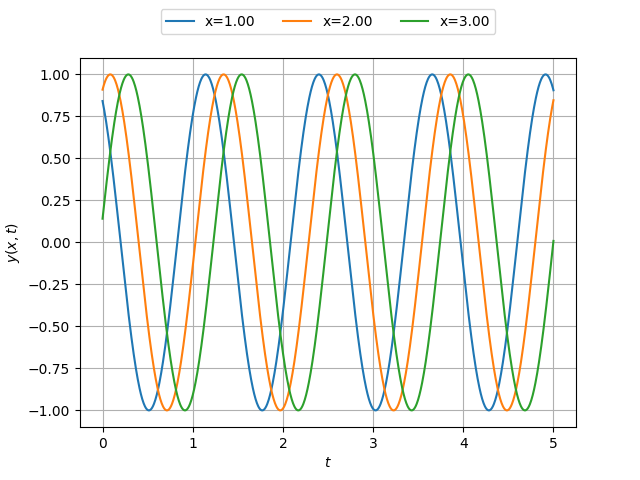
\includegraphics[width=\columnwidth]{2021/BM/28/figs/plot.png}
	\caption{Plot of $y(x,t)$}
	\label{fig:plot_bm_28}
\end{figure}

\pagebreak

\item In the circuit, switch 'S' is in the closed position for a very long time. If the switch is opened at time $t=0$, then $i_L\brak{t}$ in amperes, for $t\geq0$ is
\begin{figure}[h]
    \renewcommand\thefigure{1}
    \centering
    \begin{circuitikz}[american]
    \draw (0,0) to (1,0) to (1,-2) to [R=$4\Omega$] (3,-2) to [V=$30V$,invert] (5,-2) to (5,0) to  [R=$1\Omega$] (7,0) to [L=$0.5H$] (7,-4) to (0,-4) to [V=$10V$,invert] (0,0);
    % Draw the open switch
    \draw (1,0) to[ospst] (5,0);
    % Add a label for the open switch
    \node at (3,0.8) {\scriptsize{Open at $t=0$}};
    % Draw the arrow and label for current
    \draw [->] (6.6,-1.4) -- (6.6,-2.7);
    \node at (6.4,-1.9) {$i_{L}$};
    \end{circuitikz}
    \caption{Circuit in $T$ domain}
    \label{fig:EE_21_29_1}
\end{figure}
\\
\hfill(GATE 2021 EE 29)\\
\solution
\iffalse
\let\negmedspace\undefined
\let\negthickspace\undefined
\documentclass[journal,12pt,twocolumn]{IEEEtran}
\usepackage{cite}
\usepackage{circuitikz}
\usepackage{amsmath,amssymb,amsfonts,amsthm}
\usepackage{algorithmic}
\usepackage{graphicx}
\usepackage{textcomp}
\usepackage{xcolor}
\usepackage{txfonts}
\usepackage{listings}
\usepackage{enumitem}
\usepackage{mathtools}
\usepackage{gensymb}
\usepackage{comment}
\usepackage[breaklinks=true]{hyperref}
\usepackage{tkz-euclide} 
\usepackage{listings}
\usepackage{gvv}                                        
\def\inputGnumericTable{}                                 
\usepackage[latin1]{inputenc}                                
\usepackage{color}                                            
\newtheorem{theorem}{Theorem}[section]
\usepackage{array}                                            
\usepackage{longtable}                                       
\usepackage{calc}                                             
\usepackage{multirow}                                         
\usepackage{hhline}                                           
\usepackage{ifthen}                                           
\usepackage{lscape}
\newtheorem{problem}{Problem}
\newtheorem{proposition}{Proposition}[section]
\newtheorem{lemma}{Lemma}[section]
\newtheorem{corollary}[theorem]{Corollary}
\newtheorem{example}{Example}[section]
\newtheorem{definition}[problem]{Definition}
\newcommand{\BEQA}{\begin{eqnarray}}
\newcommand{\EEQA}{\end{eqnarray}}
\newcommand{\define}{\stackrel{\triangle}{=}}
\theoremstyle{remark}
\newtheorem{rem}{Remark}
\begin{document}
\bibliographystyle{IEEEtran}
\vspace{3cm}
\title{GATE 21 EE/29}
\author{EE23BTECH11040 - Manoj Kumar Ambatipudi$^{*}$% <-this % stops a space
}
\maketitle
\newpage
\bigskip
\renewcommand{\thefigure}{\theenumi}
\renewcommand{\thetable}{\theenumi}
\textbf{QUESTION:}
In the circuit, switch 'S' is in the closed position for a very long time. If the switch is opened at time $t=0$, then $i_L\brak{t}$ in amperes, for $t\geq0$ is
\begin{figure}[h]
    \renewcommand\thefigure{1}
    \centering
    \begin{circuitikz}[american]
    \draw (0,0) to (1,0) to (1,-2) to [R=$4\Omega$] (3,-2) to [V=$30V$,invert] (5,-2) to (5,0) to  [R=$1\Omega$] (7,0) to [L=$0.5H$] (7,-4) to (0,-4) to [V=$10V$,invert] (0,0);
    % Draw the open switch
    \draw (1,0) to[ospst] (5,0);
    % Add a label for the open switch
    \node at (3,0.8) {\scriptsize{Open at $t=0$}};
    % Draw the arrow and label for current
    \draw [->] (6.6,-1.4) -- (6.6,-2.7);
    \node at (6.4,-1.9) {$i_{L}$};
    \end{circuitikz}
    \caption{Circuit in $T$ domain}
    \label{fig:EE_21_29_1}
\end{figure}
\\
\hfill(GATE 2021 EE 29)
\textbf{Solution:}
\fi
\begin{table}[h]
\renewcommand\thetable{1}
    \centering
    \begin{tabular}{|c|c|c|}
    \hline
         Variables&Description&value  \\\hline
            $i_L\brak{0}$   &    Initial current in Inductor & 10A\\\hline
            L     & Inductance of Inductor & 0.5H\\\hline
    \end{tabular}
    \caption{Caption}
    \label{tab:EE_21_29_1}
\end{table}

Circuit in $S$ domain is
\begin{figure}[h]
\renewcommand\thefigure{2}
    \centering
    \begin{circuitikz}[american]
    \draw (0,0) to (0.9,0) to (0.9,-2) to [generic=$4\Omega$] (2.9,-2) to [V=$\frac{30}{s}V$,invert](4.9,-2) to (4.9,0) to  [generic=$1\Omega$](6.9,0) to [generic=$0.5s$](6.9,-2) to [V=$Li_L\brak{0}$,invert](6.9,-4) to (0,-4) to [V=$\frac{10}{s}V$,invert](0,0);
    \draw (0.9,0) to[ospst] (4.9,0);
    % Add a label for the open switch
    \node at (3,0.8) {\scriptsize{Open at $t=0$}};
    \end{circuitikz}
    \caption{Circuit in $S$ domain}
    \label{fig:EE_21_29_2}
\end{figure}
\\
From \figref{fig:EE_21_29_1}, $i_L\brak{0}$ can be found using steady state analysis. Writing $KVL$ , we get
\begin{align}
    10-i_L\brak{0} &= 0\\
    i_L\brak{0} &= 10\label{eq:EE_21_29_1}
\end{align}
Writing $KVL$ for \figref{fig:EE_21_29_2},
\begin{align}
    \frac{10}{s} - I_L\brak{s}\brak{4+1+0.5s} + \frac{30}{s} + Li_L\brak{0} &= 0\\
    \implies I_L\brak{s} &= \frac{sLi_L\brak{0}+40}{5s + 0.5s^2} 
\end{align}
From \tabref{tab:EE_21_29_1}, 
\begin{align}
    I_L\brak{s} &= \frac{2.5s+40}{5s + 0.5s^2}\\
    I_L\brak{s} &= \frac{10s+80}{10s + s^2}\\
                &= \frac{8}{s} + \frac{2}{s+10}
\end{align}
Taking Inverse Laplace, 
\begin{align}
    i_L\brak{t} &= \brak{8+2e^{-10t}}u\brak{t}
\end{align}
\begin{figure}[h]
\renewcommand\thefigure{3}
    \centering
    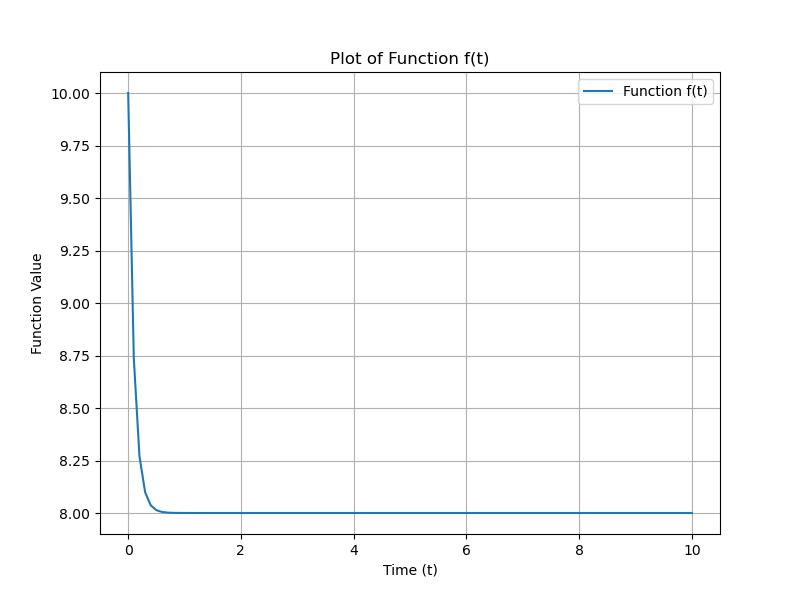
\includegraphics[width=1.0\columnwidth]{2021/EE/29/figs/fig_3.jpg}
    \caption{Plot of $i_L\brak{t}$ taken from Python3}
    \label{fig:EE_21_29_3}
\end{figure}

\pagebreak
\end{enumerate}
